\section{Methodology (Research Project Details)}


\subsection{Minutiae Extraction}


\begin{figure}[htbp]
    \centering
    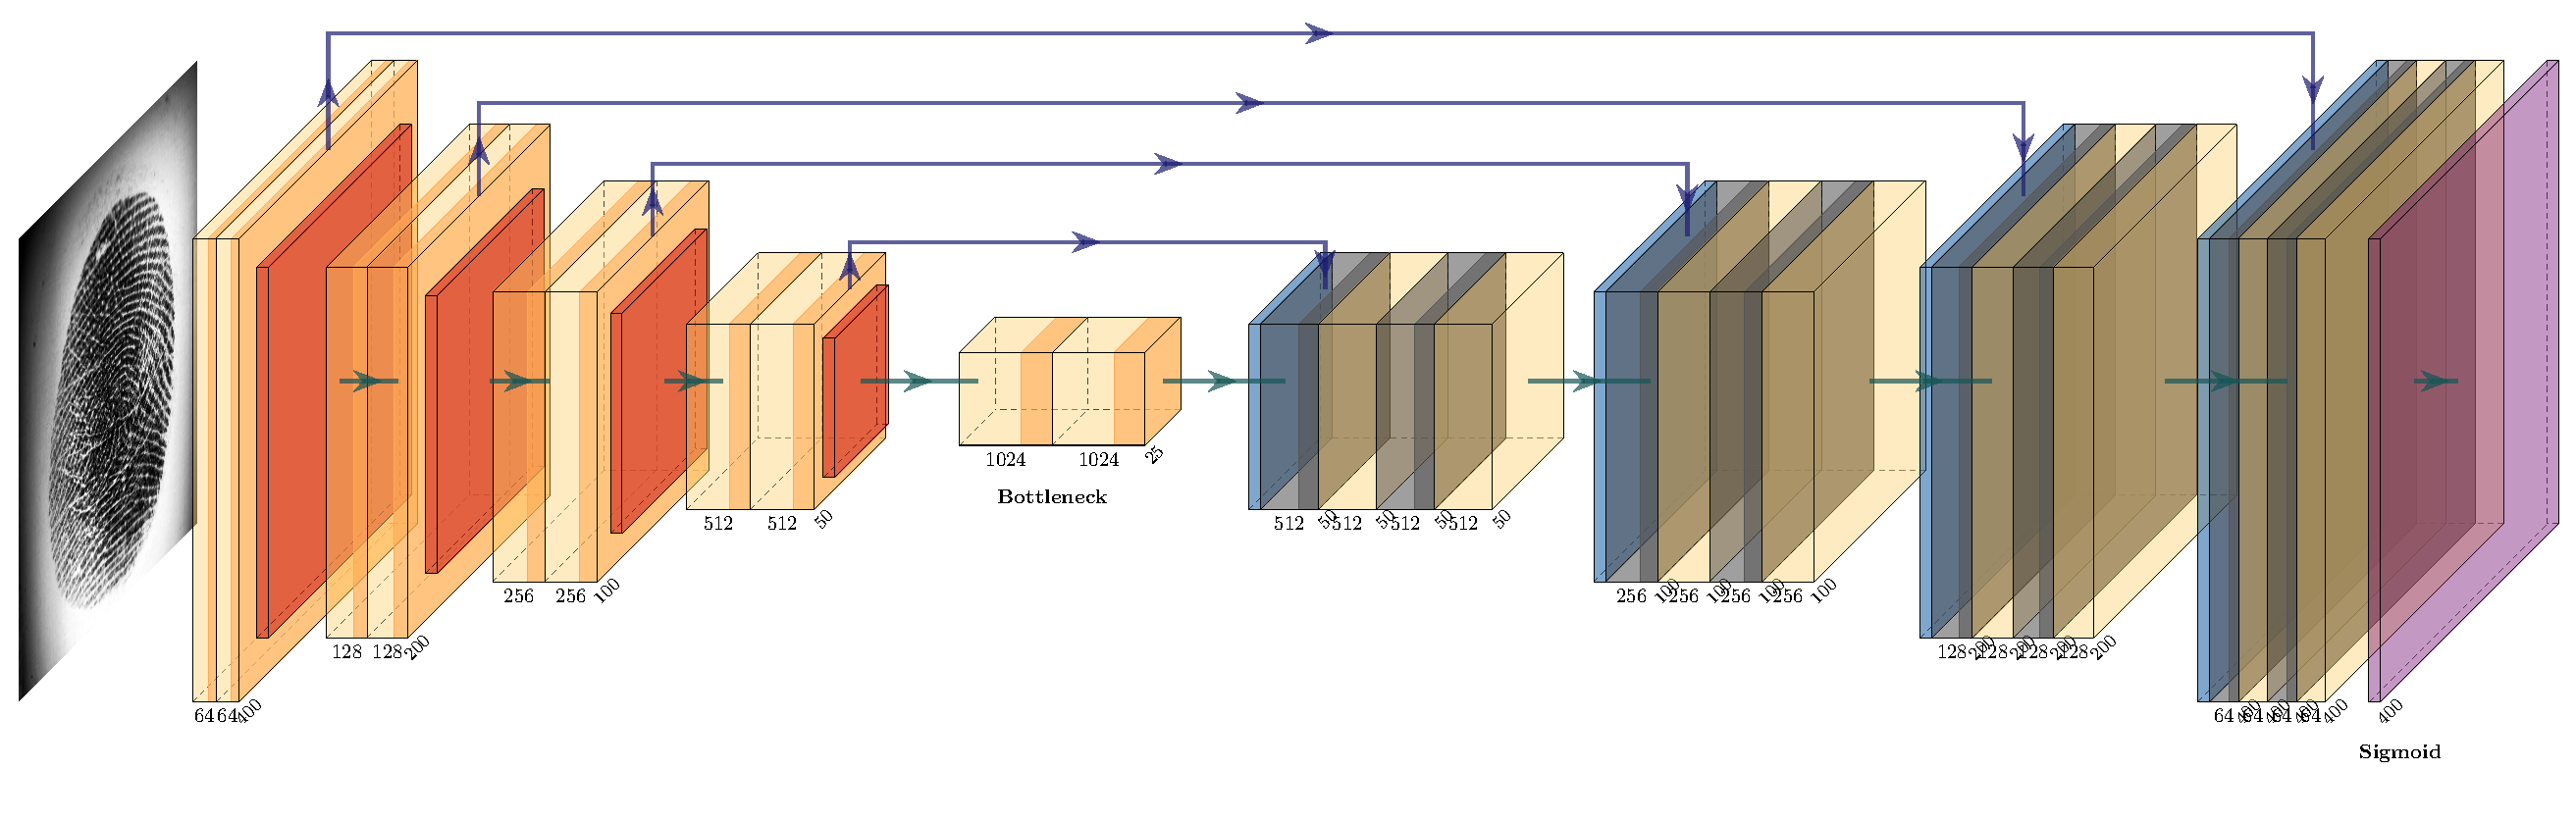
\includegraphics[width=.9\linewidth]{fig/unet.pdf}
    \caption{The structure of our minutiae feature neural network, generated with \cite{PlotNeuralNet}}
    \label{fig:unet}
\end{figure}

Fig. \ref{fig:unet} presents the basic structure of our minutiae detection network.
We input the augmented fingerprint images (with a size of $ 560*400 $ ) into the neural network and then use a UNet to extract the minutiae from it.
We use the ResNet18 as encoder or backbone and use pre-trained weights in imagenet for the backbone initialization.


\subsection{Minutiae Feature}


\subsection{Minutiae Graph Matching}


\subsection{Loss Function}


\subsection{Data Augmentation}

\begin{figure}[htbp]
    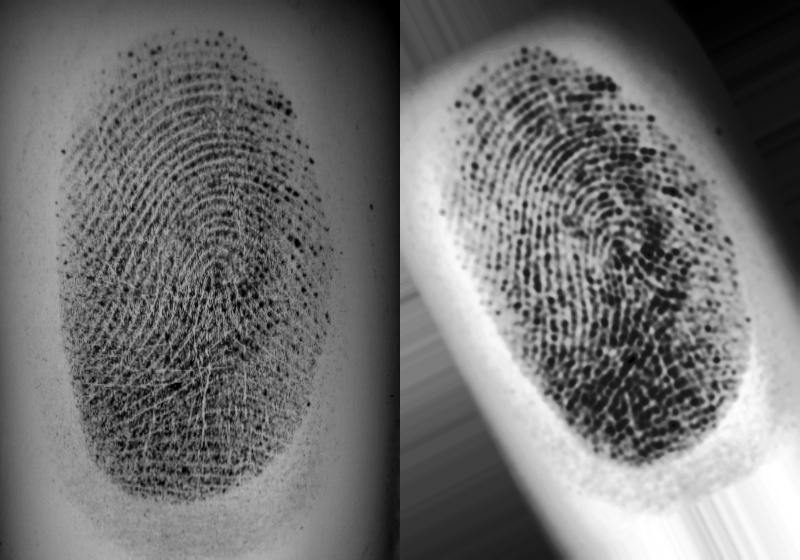
\includegraphics[width=.32\linewidth]{fig/augmentation/aug-1.jpg}
    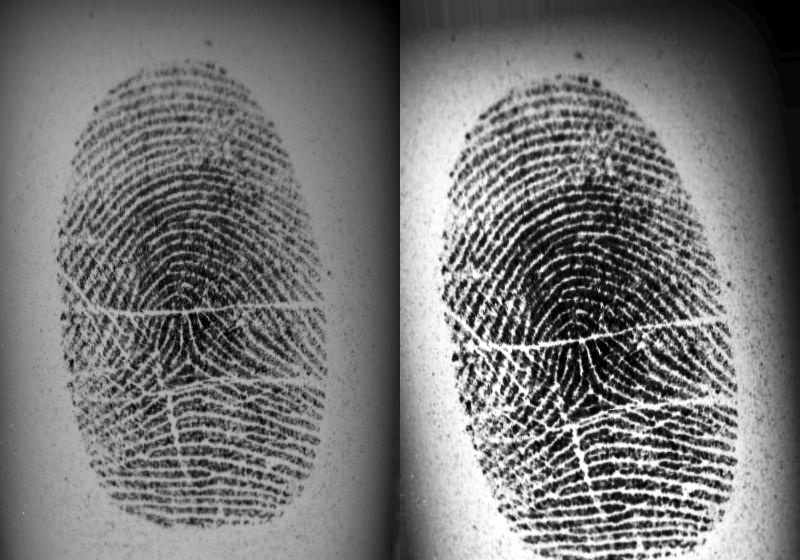
\includegraphics[width=.32\linewidth]{fig/augmentation/aug-2.jpg}
    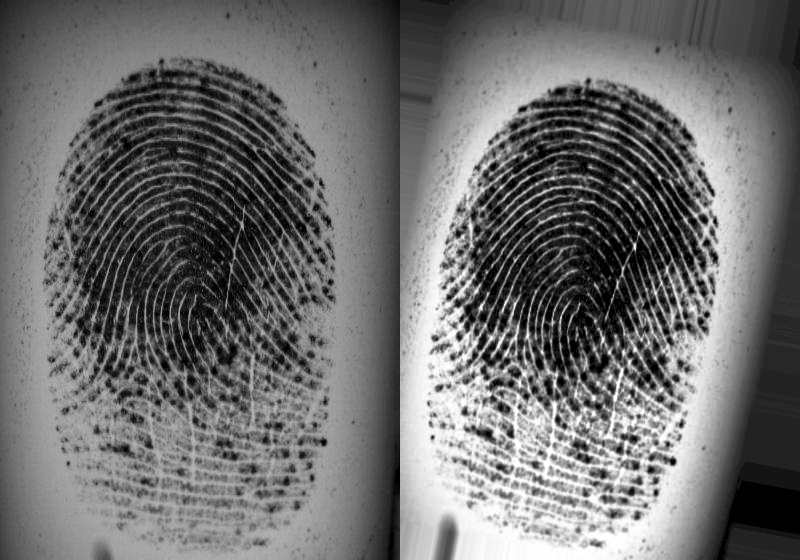
\includegraphics[width=.32\linewidth]{fig/augmentation/aug-3.jpg}
    \newline
    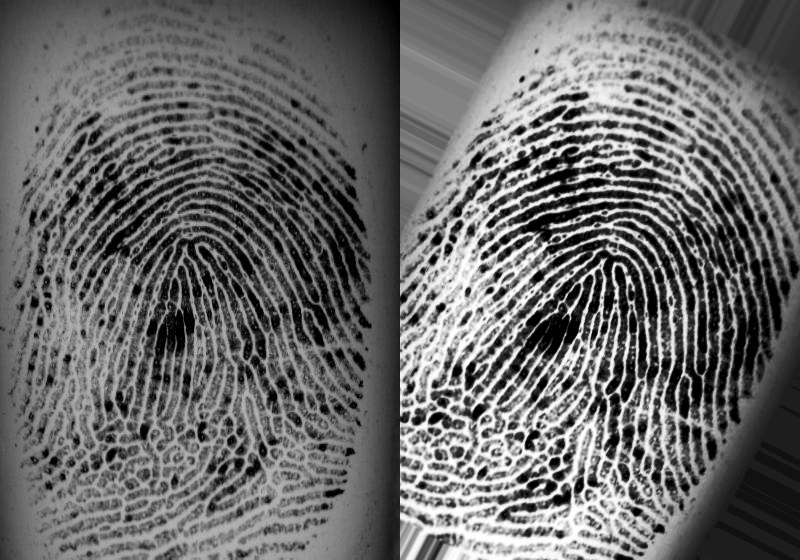
\includegraphics[width=.32\linewidth]{fig/augmentation/aug-4.jpg}
    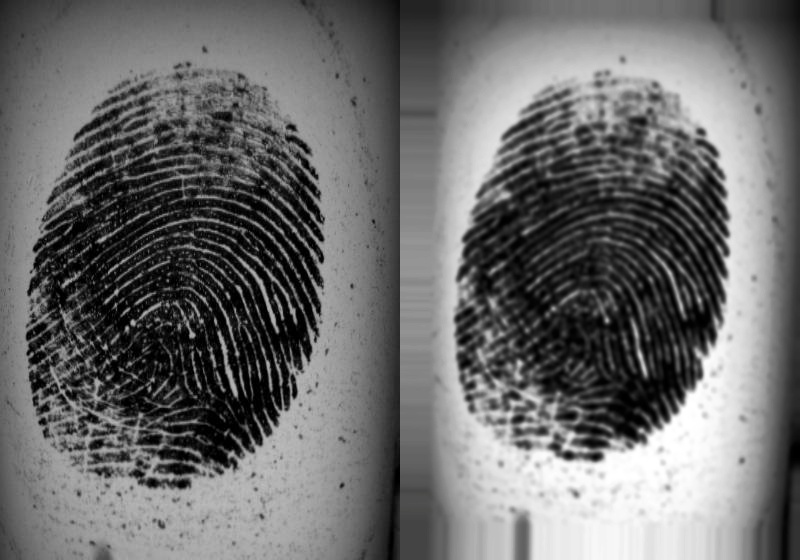
\includegraphics[width=.32\linewidth]{fig/augmentation/aug-5.jpg}
    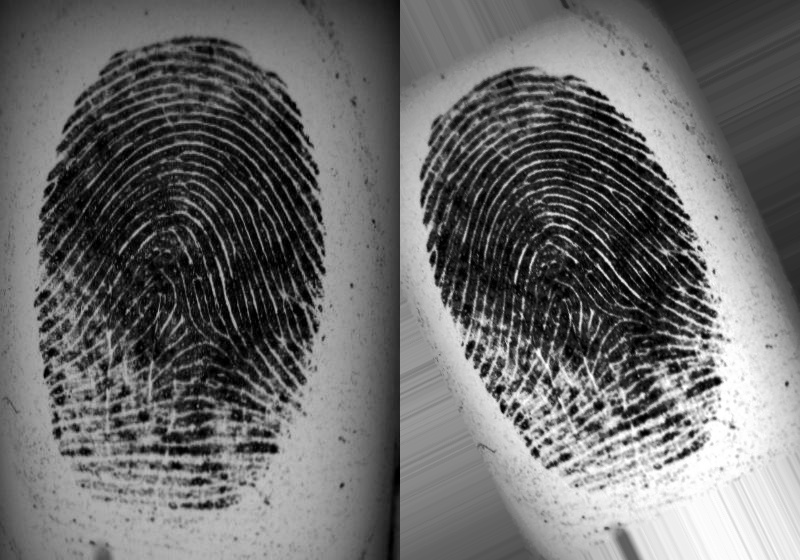
\includegraphics[width=.32\linewidth]{fig/augmentation/aug-6.jpg}
    \caption{Augmentation images samples, left are the original images while right are the augmented images}
    \label{fig:augmentation}
\end{figure}

It is worth to mention that we also do some data augmentation in our experiment to improve the robustness and accuracy.
We use imgaug \cite{imgaug} library in this experiment.
And mainly use the following transforms: random brightness, gamma contrast, Gaussian blur and shift scale rotate.
After the data augmentation, we add a histogram equalization to normalize the images.
Fig \ref{fig:augmentation} presents some sample data augmentation images pairs, where the left is the original fingerprint image and the right is the augmented image.


